\section{Simulation studies}
\label{Section:Simulation}
%
We now present the results of two simulation studies to compare the performance of our
proposed fast variable selection method using model $e$-values, with the model selection procedures obtained from backward deletion and all subset regression versions that aim to minimize the Akaike Information Criterion (AIC: \cite{Akaike70}) or the BIC for linear model, and sparse regularization-based methods for linear mixed models. In both examples below, we assume that the expectation of the response $Y$ is a linear function of a few covariates, and the model selection problem is the classical one of identifying the set of covariates which have a non-zero effect on $\BE Y$.

%We consider different ratios of the number of covariates included in the minimal adequate model and the total number of covariates. We consider two different kinds of resampling plans: the {\textit {moon-bootstrap}} ($m$-out-of-$n$ bootstrap) and one where the resampling weights used in \eqref{eq:Psisnhat_R} are independent, identically distributed Gamma random variables, which may be considered a variant of the Bayesian bootstrap and referred to as {\textit{gamma bootstrap}} below. In either case, the random variables $\BW_{r s n i}$ used in \eqref{eq:Psisnhat_R}  tend to infinity as $n \raro \infty$, which is a crucial condition for our results. In the moon-bootstrap, this variance is given by $\tau^{2}_{n} = n/m$. We examine the effect of different choices of $\tau^{2}_{n}$ in both the moon-bootstrap and the gamma-bootstrap.

\subsection{Selecting covariates in linear regression}

For the first simulation, we use the first $p = 10$ columns of a simulated dataset from Prof. Charles Geyer's website (\url{http://www.stat.umn.edu/geyer/5102/data/ex6-8.txt}) and $n = 100$ randomly chosen rows, and arrange then in a $n \times p$ covariate matrix $\bfX$. Each non-zero regression slope parameter takes the value 1, and we add independent standard Normal noise to generate the response vector, thus obtaining the 
framework $Y = \bfX \bfbeta + \epsilon$.

We generate data under different choices of the size of the minimal adequate model:b by first selecting $k \in \{ 2, 4, 6, 8 \}$, then setting the first $k$ coefficients of the regression slope $\bfbeta$ to be 1, and the rest $p - k$ slope parameters to be zero. The values of $\tau = \tau_{n} / \sqrt n$, the standard deviation of the resampling weights scaled by $\sqrt n$, is selected on a grid between 1 and 10 in 0.1 length intervals. We use a resampling Monte Carlo size $R = R_{1} = 1000$ for use in the sample version of \ref{equation:BootEValue}, Finally the entire exercise is repeated 1000 times independently. We report here the results on the proportion of times out of this 1000 replications of the study when the minimal adequate model is selected. This is the numeric approximation of the `probability of selecting the true model'.  

\begin{figure}
\begin{center}

\begin{tabular}{cc}
		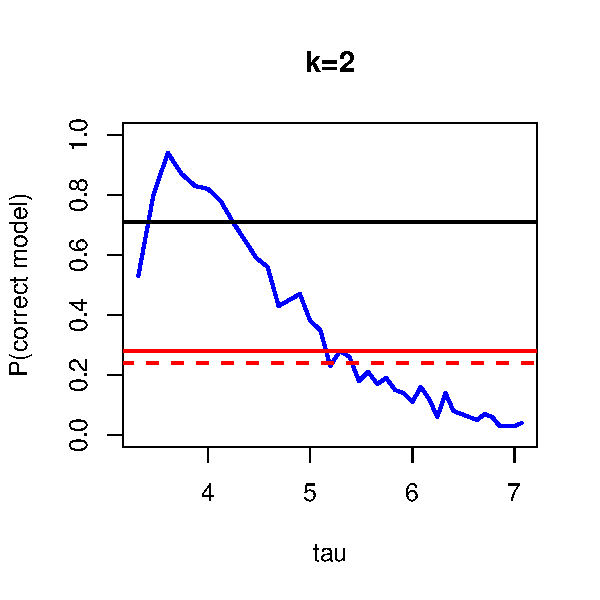
\includegraphics[width=0.32\textwidth]{Chapter-evalue/simplotmoon2}
	& 
		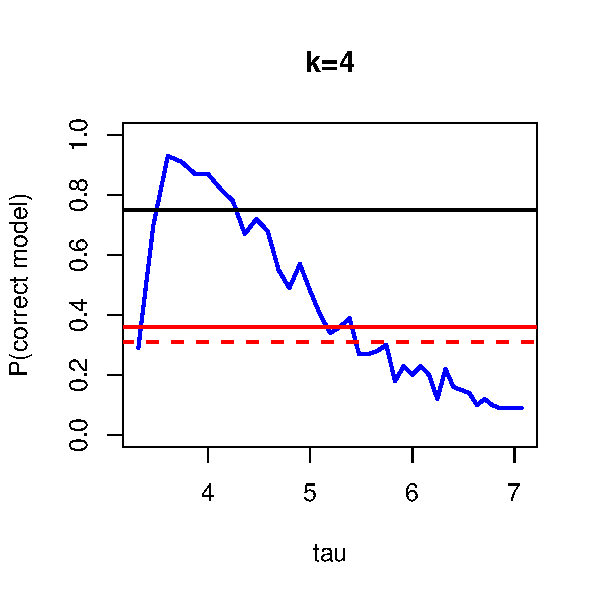
\includegraphics[width=0.32\textwidth]{Chapter-evalue/simplotmoon4} \\
	(a) & (b) \\	
		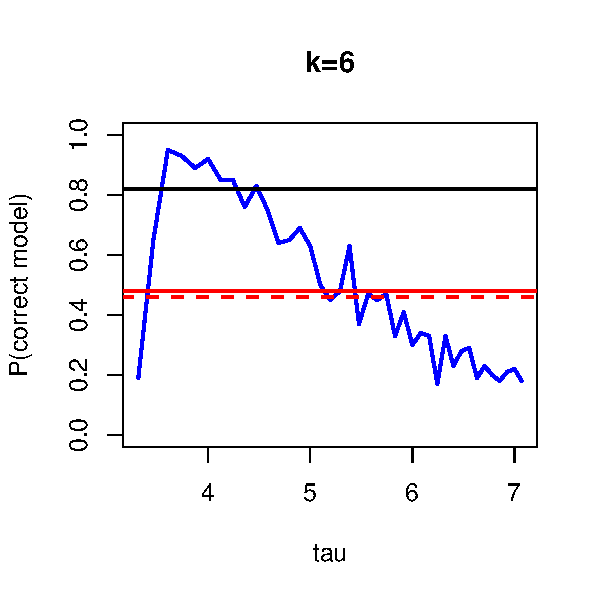
\includegraphics[width=0.32\textwidth]{Chapter-evalue/simplotmoon6}
	& 
		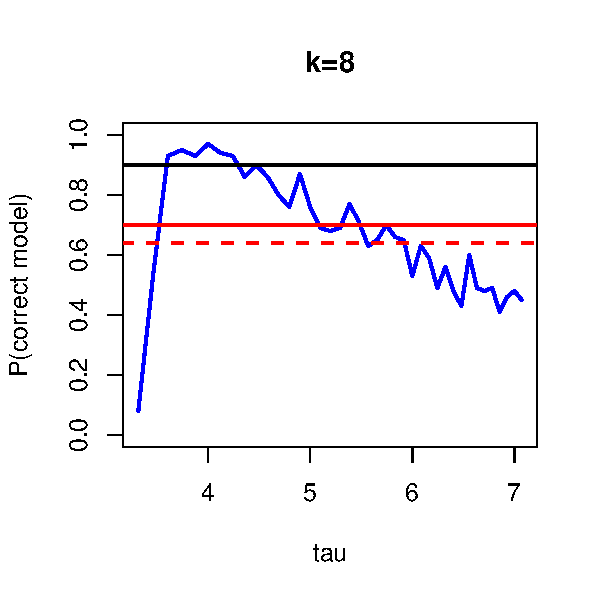
\includegraphics[width=0.32\textwidth]{Chapter-evalue/simplotmoon8} \\
	(c) & (d) \\	
\end{tabular}

\caption{Empirical probabilities of selecting the correct model through moon bootstrap for several levels of sparsity:  The $e$-values method- blue solid, AIC backward deletion- red dotted, AIC all subset- red solid, BIC backward deletion- black dotted, BIC all subset- black solid}
\label{fig:simplotsmoon}

\end{center}
\end{figure}

\begin{figure}
\begin{center}

\begin{tabular}{cc}
		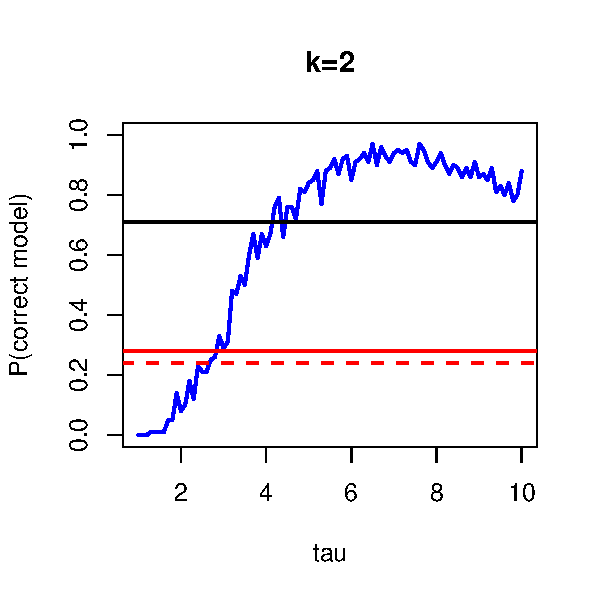
\includegraphics[width=0.32\textwidth]{Chapter-evalue/simplot_gamma2}
	& 
		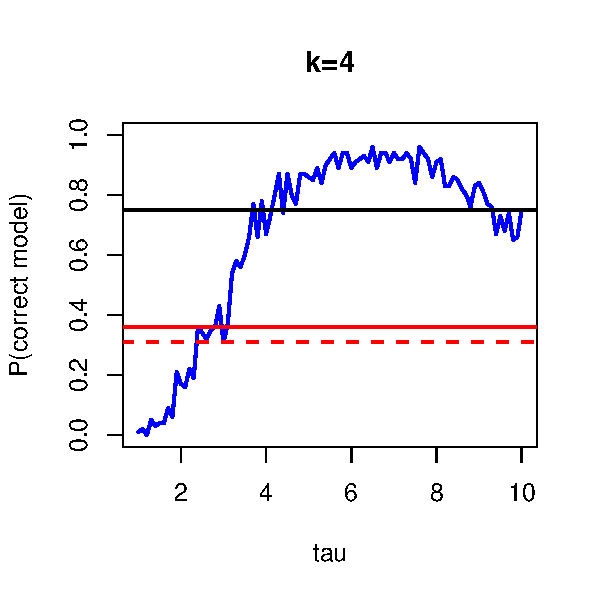
\includegraphics[width=0.32\textwidth]{Chapter-evalue/simplot_gamma4} \\
	(a) & (b) \\	
		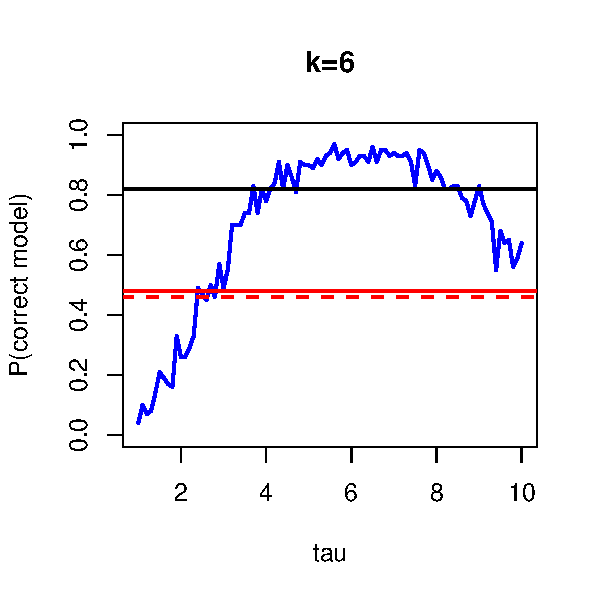
\includegraphics[width=0.32\textwidth]{Chapter-evalue/simplot_gamma6}
	& 
		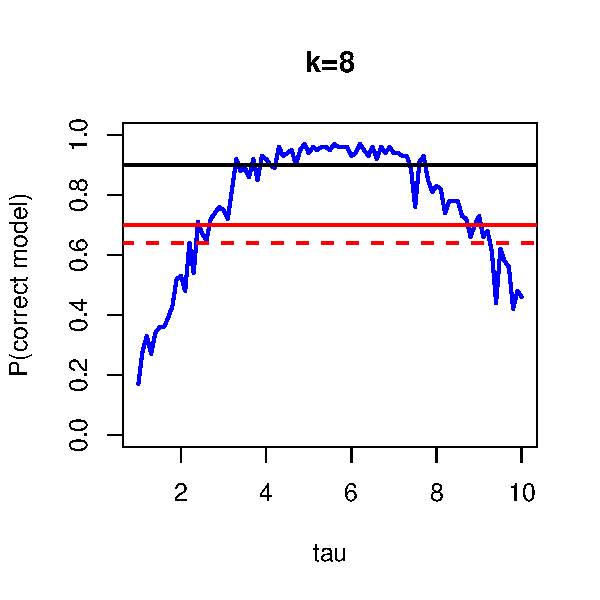
\includegraphics[width=0.32\textwidth]{Chapter-evalue/simplot_gamma8} \\
	(c) & (d) \\	
\end{tabular}

\caption{Empirical probabilities of selecting the correct model through gamma bootstrap for several levels of sparsity:  The $e$-values method- blue solid, AIC backward deletion- red dotted, AIC all subset- red solid, BIC backward deletion- black dotted, BIC all subset- black solid}
\label{fig:simplotsgamma}

\end{center}
\end{figure}

\begin{figure}
\begin{center}

\begin{tabular}{cc}
		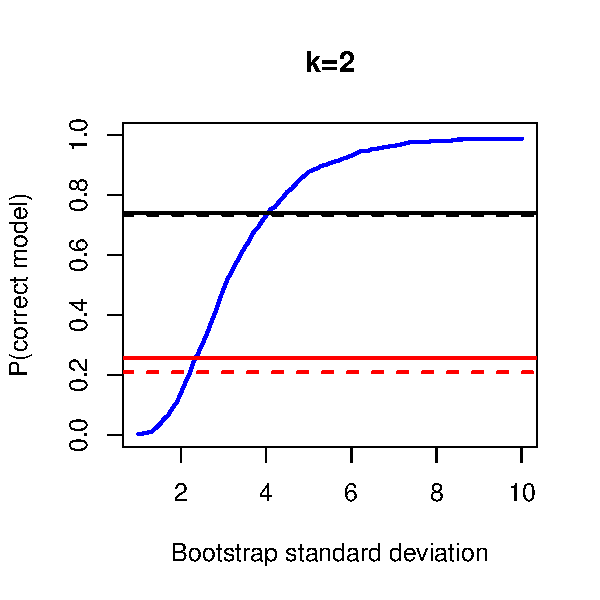
\includegraphics[width=0.32\textwidth]{Chapter-evalue/simplot2}
	& 
		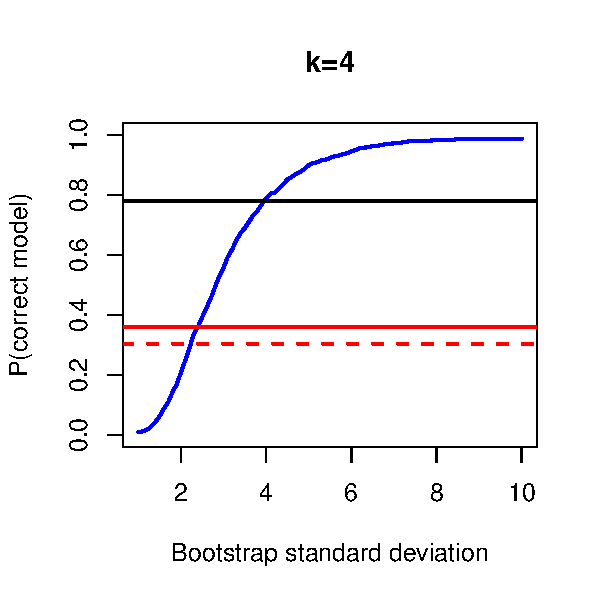
\includegraphics[width=0.32\textwidth]{Chapter-evalue/simplot4} \\
	(a) & (b) \\	
		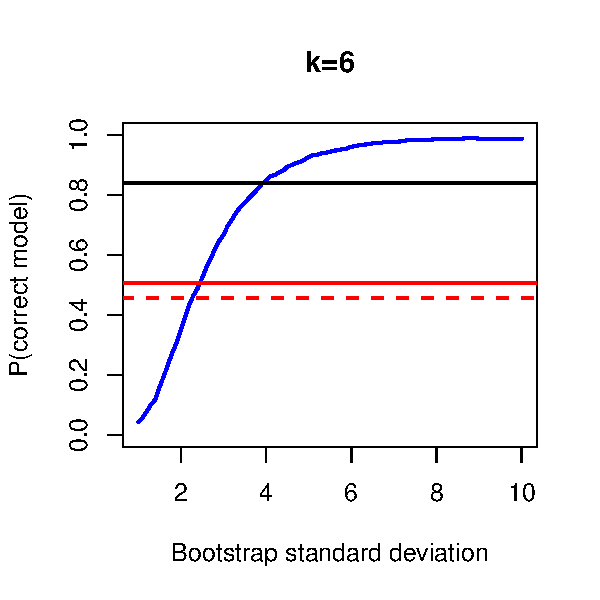
\includegraphics[width=0.32\textwidth]{Chapter-evalue/simplot6}
	& 
		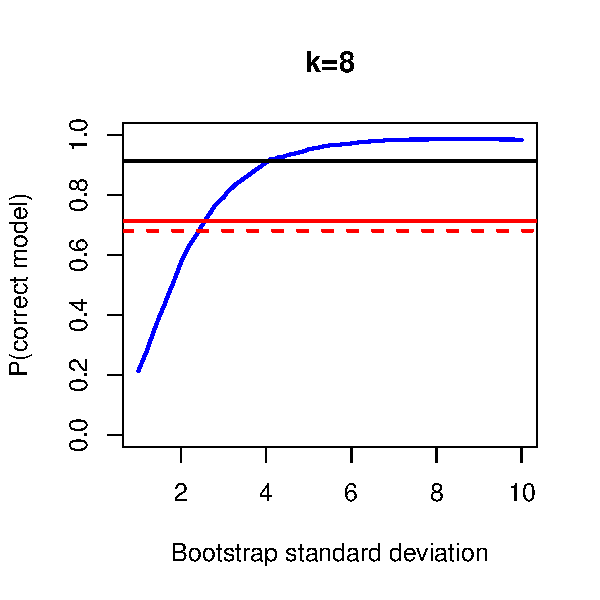
\includegraphics[width=0.32\textwidth]{Chapter-evalue/simplot8} \\
	(c) & (d) \\	
\end{tabular}

\caption{Empirical probabilities of selecting the correct model through wild bootstrap for several levels of sparsity:  The $e$-values method- blue solid, AIC backward deletion- red dotted, AIC all subset- red solid, BIC backward deletion- black dotted, BIC all subset- black solid}
\label{fig:simplotswild}

\end{center}
\end{figure}

We use the backward deletion and all-subset regression search strategies while using AIC and BIC as the model selection criterion. We use the leaps-and-bound algorithm, implemented in the {\texttt{R}} package \texttt{leaps}, for all-subset search. We display the results of this study in \ref{fig:simplotsmoon} for the moon bootstrap, in \ref{fig:simplotsgamma} for the gamma bootstrap and \ref{fig:simplotswild} for a wild bootstrap \citep{Mammen93} version of the linear regression equivalent of \ref{equation:LMMBootEqn} with i.i.d. $N(0,1)$ weights. In all three methods, and for all of $k \in \{2, 4, 6, 8 \}$ the proposed $e$-value based method performs better than AIC or BIC, as long as $\tau_{n}^{2}$ is not too small or too large. This is entirely as expected. The parametric wild bootstrap procedure has the best performance among the three, giving almost perfect detection for even very large values of $\tau_n$.
%Also interestingly, unlike the AIC or BIC, the proposed {\textit{e-value}}-based 
%procedure has the same level of accuracy in detecting the correct model regardless 
%of the amount of sparsity in $\bfbeta$. 
We experimented with other choices of $n, p, R_{1}, R_{2}$, and it seems considering $\tau \in (4, 8)$ 
in this problem ensures exact minimal adequate model selection with high chance, and typically better performance than BIC in this regard. As long as $R$ and $R_{1}$ are of the order of a few hundreds or higher, the variation from the resampling Monte Carlo step seems ignorable.

\subsection{Model selection in the presence of random effects}
Here we use the repeated measures simulation setup from \cite{PengLu12}, which has 9 fixed effects and 4 random effects, with true $\bfbeta = (0,1,1,0,0,0,0,0,0)$ and random effect covariance matrix:
%
\begin{align*}
D = \left(
	\begin{tabular}{cccc}
		9 & ~ & ~ & ~\\
		4.8 & 4 & ~ & ~\\
		0.6 & 1 & 1 & ~\\
		0 & 0 & 0 & 0\\
	\end{tabular}
	\right)
\end{align*}	
%
The error variance $\sigma^2$ is set at 1. The goal is to select the covariates of the fixed effect, thus essentially identify the covariates corresponding to the entries where $\bfbeta$ is non-zero. We use two scenarios for our study: one where the number of subjects considered is $m = 30$,  and the number of observations per subject is $n_i = 5$, and another with 60 subjects and 10 observations per subject.

%The model for the $i^\text{th}$ subject can be written as:
%%
%$$ \bfy_i = X_i \bfbeta + \bfepsilon_i $$
%%
%where $\bfepsilon_i \sim \mathcal N_{n_i} ({\bf 0}, \sigma^2 I + Z_i D Z_i^T)$. We use wild bootstrap on these residuals, so that the bootstrap equivalent of the response will be $\bfy_i^b = X_i \hat\bfbeta_{n,\text{LMM}} + u_{ib} (\bfy_i - X_i \hat\bfbeta_{n,\text{LMM}})$; with $u_{ib} \sim N(0, \tau^2)$. We take the bootstrap standard deviation $\tau = 1,2,...,8$, and determine the accuracy of our method by four measures: 

We consider $\tau \in \{1, \ldots, 15 \}$ here, and use the approximation in \ref{equation:LMMBootEqn} to calculate the bootstrapped coefficients. We consider multiple characteristics of the model that obtains the highest $e$-value, including the number of parameters it involves, the proportion of times the minimal adequate model is 
obtained, the proportion of times a zero-valued (non-zero-valued) element of beta was identified as non-zero (zero), that is, the proportion of false positives (negatives), and so on.   

In the method proposed by \cite{PengLu12}, the tuning parameter can be selected using several different criteria. We present the false positive percentage (FPR\%), false negative percentage (FNR\%) and model sizes corresponding to 
four such criteria. Our results are presented in  \ref{table:simtable1}. It can be seem the $e$-value based method handsomely outperforms the  method proposed by \cite{PengLu12}, especially in smaller sample sizes, as long as $\tau \geq 4$. 

\begin{table}[t]
	\centering
	\begin{scriptsize}
   \begin{tabular}{ll|lll|lll}
    \hline
    Method      & Tuning     & FPR\% & FNR\% & Model size & FPR\% & FNR\% & Model size \\ \cline{3-8}
    ~ & ~ & \multicolumn{3}{l|}{$n_i=5,m=30$} & \multicolumn{3}{l}{$n_i=10,m=60$}\\ \hline
  $e$-value based       & $\tau=1$      & 59.9     & 0.0   & 5.61       & 44.3     & 0.0   & 4.43       \\
    ~      & $\tau=2$      & 33.0     & 0.0   & 3.45       & 15.5     & 0.0   & 2.54       \\
    ~      & $\tau=3$      & 15.9     & 0.0   & 2.59       & 5.2      & 0.0   & 2.17       \\
    ~      & $\tau=4$      & 8.0      & 0.0   & 2.28       & 2.8      & 0.0   & 2.09       \\
    ~      & $\tau=5$      & 5.2     & 0.0   & 2.18       & 2.0   & 0.0   & 2.06       \\
    ~      & $\tau=6$      & 2.7     & 0.0   & 2.09       & 0.7   & 0.0   & 2.02       \\
    ~      & $\tau=7$      & 2.2   & 0.0   & 2.07       & 0.3   & 0.0   & 2.01       \\
    ~      & $\tau=8$      & 1.5   & 0.0   & 2.05       & 0.3   & 0.0   & 2.01       \\
    ~      & $\tau=9$      & 1.0   & 0.0   & 2.03       & 0.3   & 0.0   & 2.01       \\
    ~      & $\tau=10$      & 0.7   & 0.0   & 2.02       & 0.3   & 0.0   & 2.01       \\
    ~      & $\tau=12$      & 0.7   & 0.0   & 2.02       & 0.0   & 0.0   & 2.00       \\
    ~      & $\tau=15$      & 0.7   & 0.0   & 2.02       & 0.0   & 0.0   & 2.00       \\
     \hline
    \cite{PengLu12} & BIC    & 21.5  & 9.9   & 2.26       & 1.5   & 1.9   & 2.10       \\
    ~      & AIC    & 17    & 11.0  & 2.43       & 1.5   & 3.3   & 2.20       \\
    ~      & GCV    & 20.5  & 6     & 2.30       & 1.5   & 3     & 2.18       \\
    ~      & $\sqrt{\log n/n}$ & 21    & 15.6  & 2.67       & 1.5   & 4.1   & 2.26       \\ \hline
    \end{tabular}
    \caption{Comparison between our method and that proposed by \cite{PengLu12} through average false positive percentage, false negative percentage and model size}
    \label{table:simtable1}
    \end{scriptsize}
\end{table}
%
\begin{table}[t]
	\centering
	\begin{scriptsize}
    \begin{tabular}{llll}
    \hline
    Method          & ~ & Setting 1 & Setting 2 \\ \hline
    $e$-value based     & $\tau=1$ & 3         & 14       \\
    ~               & $\tau=2$ & 30      & 60        \\
    ~               & $\tau=3$ & 61        & 86      \\
    ~               & $\tau=4$ & 79        & 92      \\
    ~               & $\tau=5$ & 87        & 94       \\
    ~               & $\tau=6$ & 93      & 98       \\
    ~               & $\tau=7$ & 94       & 99       \\
    ~               & $\tau=8$ & 96       & 99       \\
    ~               & $\tau=9$ & 97       & 99       \\
    ~               & $\tau=10$ & 98       & 99       \\
    ~               & $\tau=12$ & 98       & 100       \\
    ~               & $\tau=15$ & 98       & 100       \\\hline
    \cite{BondellKrishnaGhosh10} & ~ & 73        & 83        \\
    \cite{PengLu12}         & ~ & 49        & 86        \\
    \cite{FanLi12}           & ~ & 90        & 100       \\ \hline
    \end{tabular}
    \caption{Comparison of our method and three sparsity-based methods of mixed effect model selection through accuracy of selecting correct fixed effects}
	\label{table:simtable2MS}
    \end{scriptsize}
\end{table}

We also compare the percentages of times the correct model was identified, and these results are presented in \ref{table:simtable2MS}, along with the corresponding results from two other papers. The proposed $e$-value based procedure performs best here for $\tau \geq 6$ for the smaller sample setting, and for $\tau\geq 12$ for larger sample setting. 

